\documentclass[12pt,openany,a4paper, titlepage]{article}

%import package
\usepackage[utf8]{inputenc}
\usepackage[T1]{fontenc}
\usepackage{lmodern}
\usepackage[french]{babel}
\usepackage{amsfonts,amsmath,amssymb,amsthm}
\usepackage{geometry} %fix the margin of the document
\geometry{top=3cm, bottom=3cm, left=2.5cm, right=2.5cm}
\usepackage{xargs}    %define new command
\usepackage{graphicx} %insertion image
\usepackage{caption}  %insertion de légendes et titres
\usepackage{indentfirst}
\usepackage{color}
\usepackage[table]{xcolor}
\usepackage{float}
\usepackage{tcolorbox}
\usepackage{appendix} % Appendices

% Bibliographie
\usepackage[backend=biber,sorting=nyt,citestyle=numeric,bibstyle=alphabetic]{biblatex}% Bibliographie
\addbibresource{biblio.bib} 
\usepackage{csquotes}
\usepackage{url}

%title shape %\MakeUppercase
\usepackage{titlesec}
\titleformat{\chapter}[display]
{\normalfont\huge\bfseries\center}{\chaptertitlename\ \thechapter}{20pt}{\Huge}
\titleformat{\section}
{\normalfont\Large\bfseries\center}{\thesection}{1em}{}
\titleformat{\subsection}
{\normalfont\large\center}{\thesubsection}{1em}{}
\titleformat{\subsubsection}
{\normalfont\normalsize\bfseries\center}{\thesubsubsection}{1em}{}
\titleformat{\paragraph}[runin]
{\normalfont\normalsize\bfseries}{\theparagraph}{1em}{}
\titleformat{\subparagraph}[runin]
{\normalfont\normalsize\bfseries}{\thesubparagraph}{1em}{}

%news commands
\newcommand{\f}[2]{\frac{#1}{#2}}
\newcommand{\lp}{\left(}
\newcommand{\rp}{\right)}
\newcommand{\lb}{\left|}
\newcommand{\rb}{\right|}
\newcommand{\lc}{\left[}
\newcommand{\rcc}{\right]}
\newcommand{\la}{\left\langle}
\newcommand{\ra}{\right\rangle}
\newcommand{\dd}{\;\mathrm{d}}
\newcommand{\ddt}[1]{\frac{\partial #1}{\partial t}}
\newcommand{\R}{\mathbb{R}}
\newcommand{\C}{\mathbb{C}}
\newcommand{\Z}{\mathbb{Z}}
\newcommand{\N}{\mathbb{N}}
\newcommand{\HH}{\mathcal{H}}
\newcommand{\KK}{\mathcal{K}}
\newcommand{\spec}{\operatorname{spec}}
\newcommand{\res}{\operatorname{res}}
\newcommand{\specp}{\operatorname{spec_p}}
\newcommand{\essran}[1]{\operatorname{ess_{#1}ran}}
\newcommand{\esssup}[1]{\operatorname{ess_{#1}sup}}
\newcommand{\rd}{\mathbb{R}^d}
\newcommand{\vp}{\varphi}
\newcommand{\He}{H(\epsilon)}
\newcommand{\inv}{^{-1}}
\newcommand{\St}[2]{e^{-i #1 #2}}
\newcommand{\Stt}[2]{e^{i #1 #2}}
\newcommand{\ortho}{P^\perp}
\newcommand{\Ker}{\operatorname{Ker}}
\newcommand{\im}{\operatorname{Im}}
\newcommand{\pvm}{\mathrm{d}\langle \rangle}
\newcommand{\suminf}[2]{\sum_{#1=#2}^{+\infty}}
\newcommand{\limeo}{\lim\limits_{\epsilon \rightarrow 0^+}}

%new sections
\newtheorem{Def}{Définition}
\newtheorem{defprop}{Définition/Proposition}
\newtheorem{prop}{Proposition}
\newtheorem{theo}{Théorème}
\newtheorem{lem}{Lemme}
\theoremstyle{definition}
\newtheorem{ass}{Hypothèses}
\newtheorem{cor}{Corollaire}
\theoremstyle{definition}
\newtheorem{Not}{Notation}
\theoremstyle{definition}
\newtheorem{ex}{Exemple}
\theoremstyle{definition}
\newtheorem{exs}{Exemples}
\theoremstyle{definition}
\newtheorem{rem}{Remarque}
\newtheorem{postulat}{Postulat}
\theoremstyle{definition}

\everymath{\displaystyle}

\title{La règle d'or de Fermi}
\author{Théo Duez }

%\begin{figure}
%    \begin{minipage}[c]{.46\linewidth}
%       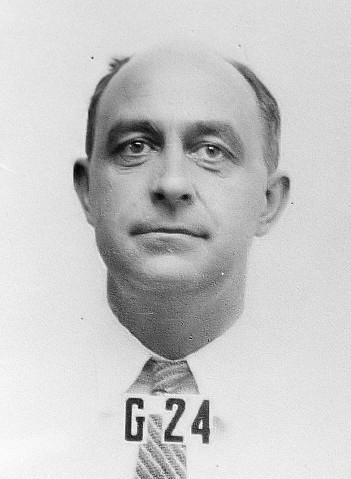
\includegraphics[height=6cm]{Enrico_Fermi.png} 
%        \caption{"Enrico Fermi"}
%    \end{minipage} \hfill
%    \begin{minipage}[c]{.46\linewidth}
%        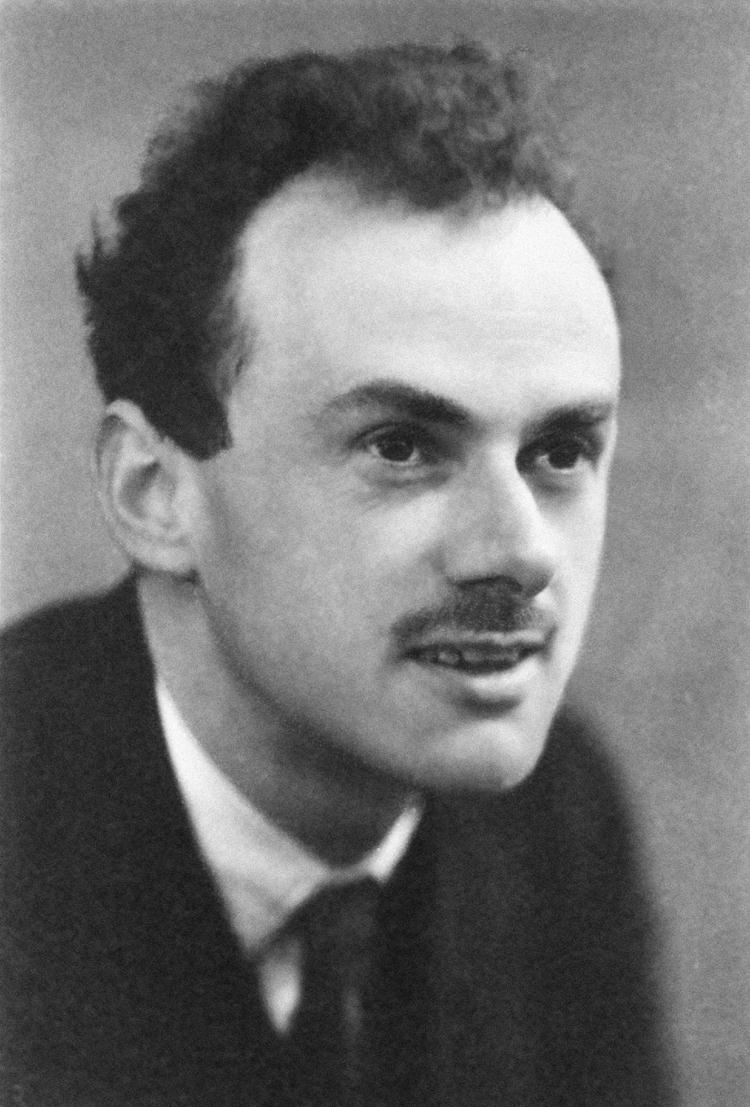
\includegraphics[height=6cm]{Paul_Dirac.jpg}
%        \caption{"Paul Dirac"}
%    \end{minipage}
%\end{figure}


\begin{document}


\maketitle

\newpage

\tableofcontents

\newpage

\section{Introduction}

\subsection{Modélisation mathématique de la mécanique quantique}

Développé dans les années par une dizaine de physiciens devenus célèbres dont notamment Paul Dirac, Werner Heisenberg, Louis de Broglie, Erwin Schrödinger etc.,  la mécanique quantique est la branche de la physique théorique qui permet d'expliquer le comportement des particules élémentaires, des atomes, des molécules ou de tout système physique de taille similaire. Elle a rencontré de nombreux succès en permettant d'expliquer ce que la physique classique ne pouvait pas, par exemple la structure électronique des atomes et des molécules, .... . 

Nous ne prétendons pas ici à fournir ne serait-ce qu'une introduction d'introduction d'un vrai cours de mécanique quantique, et bon nombre de concepts et de résultats élémentaires seront omis. Pour plus de détails, nous renvoyons le lecteur à [], [] ou []. Nous allons juste nous concentrer sur ce que l'on appelle les postulats de la mécanique quantique qui permettent de poser les bases de la modélisation mathématique et de ses outils avec lesquels nous allons traiter tout au long de ce rapport.

\vspace{3mm}
\begin{tcolorbox}[colback=gray!5!white,
                  colframe=gray!80!white,
                  title= Postulat 1 : Principe de superposition ]
L'état d'un système quantique est défini à tout instant $t$ par un vecteur unitaire, dénoté $|\psi(t)\rangle$, appartenant à un espace de Hilbert complexe $\HH$ séparable. Deux états qui différent d'un facteur de phase $e^{i\theta}$ pour $\theta\in[0,2\pi)$ représentent le même état.
\end{tcolorbox}
\vspace{3mm}

\begin{rem}
    Il est usuel en mécanique quantique de noter un vecteur 
    de $\HH$ aussi bien $\psi$ que $|\psi\rangle$. Il s'agit d'un "ket". En notant la forme linéaire associé à ce vecteur par $\langle\psi |$, i.e l'application $u\in\HH \mapsto \langle \psi | u\rangle$ appelé un "bra", on obtient que les notations coïncident avec le produit scalaire et sont très utiles en pratique. Par exemple, le projecteur sur la droite vectoriel engendrée par $|\psi\rangle$ est $|\psi\rangle\langle\psi |$.
\end{rem}

\begin{exs}
    Donnons quelques exemples d'espaces d'états.
    \begin{enumerate}
        \item[1] $\C$ est l'espace de Hilbert séparable le plus simple que l'on puisse considérer. Comme deux complexes de module 1 différent toujours d'un facteur de phase, cet espace est trivial puisque constituer que d'un seul état.
        \item[2] $\C^2$ est quant à lui l'espace non trivial le plus simple que l'on puisse considérer. Soit $|\psi\rangle = (re^{i\vp}, r'e^{i\vp'}) \in \C^2$ avec $r,r'\geq 0$ et $\vp, \vp' \in [0,2\pi)$. Quitte à multiplier par le facteur de phase $e^{-i\vp}$ (qui ne change pas l'état du système, on peut supposer $\vp = 0$. Comme un vecteur d'état est de norme 1, on a que $r^2 + r'^2 = 1$ et il existe donc $\theta \in [0,2\pi[$, que l'on peut réduire à $\theta \in [0,\pi[$ une nouvelle fois par invariance par multiplication par un facteur de phase, tel que $|\psi\rangle = \lp \cos(\theta), \sin(\theta)e^{i\vp'}\rp$. Une telle paramétrisation fait que l'on appelle cet espace d'état la sphère de Bloch, qui permet de modéliser par exemple les qubits, composants de base en théorie de l'information quantique.
        \item[3] De même, on peut considérer $\C^n$ pour $n\in\N$. Un tel espace peut modéliser un système qui peut se déplacer/propager sur un ensemble de $n$ sites.
        \item[4]  De façon plus général, si l'on souhaite considérer un système qui évolue sur une chaîne discrète infinie, l'espace approprié à considérer est $\ell^2(\Z)$, l'espace des suites sur $\Z$ de carré intégrable, qui est bien, muni sa norme euclidienne, un espace de Hilbert séparable. On peut aussi considérer $\ell^2(A)$ où $A$ est un ensemble dénombrable.
        \item[5] Un dernier exemple est l'espace $L^2(\R^d,\C)$ où $d\in\N$, l'espace des fonctions de $R^d$ vers $\C$ de carré intégrable. Cet espace est un espace de Hilbert séparable pour sa norme euclidienne. C'est l'espace typique utiliser si l'on souhaite par exemple modéliser un système dont la position varie dans un continuum, ici $\R^d$.
    \end{enumerate}
\end{exs}

\begin{rem}
    Expliquons pourquoi on demande à ce que $|\psi(t)\rangle$ soit de norme constante égale à $1$ au cours du temps. Cela est due au fait bien connue que la mécanique quantique est une description probabiliste de la physique. Si par exemple $\HH = \ell^2(A)$, on doit donc avoir $||\psi(t)||^2 = \sum_{a\in A} |\psi_a(t)|^2$ et si ou bien $\HH = L^2(\R^d,\C)$, on doit avoir $\int_{\R^d}|\psi(t,x)|^2dx = 1$. Dans le premier cas, on doit penser $|\psi_a(t)|^2$ une probabilité sur l'atome (au sens mathématique) $\{a\}$ et $|\psi(t,x)|^2$ plutôt la une densité de probabilité au point $x \in \R^d$. La position moyenne d'une particule se mouvant dans $A$ s'écrit donc par théorème de transfert $\sum_{a\in A} a|\psi_a(t)|^2$ et si elle se meut dans $\R^d$ elle s'écrit $\int_{\R^d}x|\psi(t,x)|^2dx$.
\end{rem}

\vspace{3mm}
\begin{tcolorbox}[colback=gray!5!white,
                  colframe=gray!80!white,
                  title= Postulat 2 : Principe de correspondance ]
A tout observable classique correspond un opérateur linéaire $A$ autoadjoint sur $\HH$.
\end{tcolorbox}
\vspace{3mm}

\begin{rem}
    $A$ est simplement une matrice si $\HH$ est de dimension finie mais peut être un opérateur possiblement non borné si $\HH$ est de dimension infinie. L'étude de tels opérateurs, et à l'instar des matrices de leur spectre et diagonalisabilité, fait l'objet de la théorie dite spectrale dont nous ferons un très rapide tour dans la section suivante. Ici autoadjoint est une généralisation à la dimension infinie de la notion d'hermitianité pour les matrices complexes.
\end{rem}

\begin{ex} 
Donnons quelques exemples pour des systèmes vivant dans l'espace le plus intéressant, $L^2(\R^d,\C)$ où $d\in\N$. A titre d'exemple, considérons que le système est constitué d'un électron libre.
\begin{enumerate}
    \item[1] Parler de la position, au sens classique, de l'électron en mécanique quantique n'a pas de sens puisque l'état d'un système est représenté uniquement par un vecteur $|\psi\rangle$ de l'espace de Hilbert $\HH$, ici une fonction définie sur tout $\R^d$. C'est d'ailleurs pourquoi on entend parler en mécanique quantique du "nuage électronique". En mécanique quantique, la position est un opérateur $X$ définie comme $$X|\psi\rangle = x\in \R^d \mapsto x|\psi\rangle(x) \in \C$$ de sorte qu'avec la remarque précédente, la position moyenne s'écrit $$ \langle \psi | X | \psi \rangle.$$ En fait, on appelle moyenne de l'observable $A$, la quantité $\langle \psi | A | \psi \rangle$, ce qui justifie la définition de l'opérateur position. On remarque que l'opérateur $X$ est bien un opérateur autoadjoint : soit $\psi_1, \psi_2 \in \HH$
    \begin{equation}
        \la\psi_1, X\psi_2\ra =\int_{\R^d}\overline{\psi_1(x)}x\psi_2(x) \dd x
        = \int_{\R^d}\overline{x\psi_1(x)}\psi_2(x) \dd x 
        = \la X\psi_1, \psi_2\ra.
    \end{equation}
    \item[2] De même, parler du moment (masse $\times$ vitesse) de l'électron n'a pas de sens. Quelle définition peut-on donner à l'opérateur $P$ correspondant ? L'idée naturelle est de poser que les quantités moyennes "vérifient" les principes classiques, ici que la dérivée de la position est égale au moment (en se plaçant dans un système d'unité où la masse $m$ de l'électron est telle que $m=1$ :
    $$ \langle \psi |P|\psi\rangle = m\frac{\dd \langle \psi | X | \psi\rangle}{\dd t}.$$
    \begin{theo}[Théorème d'Ehrenfest]
        Si $A$ est un opérateur autoadjoint de $\HH$ indépendant du temps, alors pour tout $\psi\in\HH$
        \begin{equation}
            \frac{\dd \langle \psi | A | \psi\rangle}{\dd t} = \psi | A | \psi\rangle
        \end{equation}
    \end{theo}
\end{enumerate}
\end{ex}


\vspace{3mm}
\begin{tcolorbox}[colback=gray!5!white,
                  colframe=gray!80!white,
                  title= Postulat 3 : Principe de quantification ]
Quelque soit l'état du système, la mesure d'une observable $A$ ne peut être qu'une valeur propre de l'observable $A$.
\end{tcolorbox}
\vspace{3mm}

\begin{rem}
    Lorsque l'on parle ici de mesure, il s'agit bien là d'une mesure physique réalisé à l'aide d'instruments et sous intervention humaine, ce qui est un point déroutant en mécanique quantique. 
\end{rem}

\begin{rem}
    Une remarque importante doit être faite concernant le spectre des opérateurs. S'il est aisé d'étudier le spectre des matrices, étudier le spectre d'opérateur de dimension infinie et possiblement non borné est beaucoup plus délicat et se traite dans des cours de théorie spectrale. Dans la section suivante, nous passerons en revue les résultats principaux sans pour autant les justifier. Donnons ici quelques aperçus. Ce qui fait que l'analyse spectrale en dimension infinie est beaucoup plus délicate et due au fait de la présence de phénomènes complètement absents en dimension finie. Déjà, une première difficulté vient de la définition du spectre. Le spectre d'une matrice carré $M$ peut être définie comme l'ensemble des complexes tel que $M-z$ ne soit pas inversible. C'est aussi équivalent à demander que $M-z$ ne soit pas subjective, ou encore pas injective. En dimension infinie, aucune des ces définitions n'est équivalentes. Le spectre est donc constitué de plusieurs parties, chacun correspondant à une facette du problème qui empêche $H-z$ d'être inversible (et d'inverse borné). Une partie de ce spectre, noté , $\sigma(H)$ressemble à celui que l'on connaît en dimension finie : les valeurs propres de multiplicité finie, constituant le spectre dit discret et noté $\sigma_d(H)$. Mais il y a aussi les valeurs propres de multiplicité infinie qui corresponde au cas d'un point d'accumulation. Les valeurs propres empêchent $H-z$ d'être injective. Une partie du spectre empêche cette quantité d'être surjective et dedans comprend un spectre continue, par exemple un intervale de $\R$
\end{rem}

\begin{exs}
    Donnons plusieurs exemples.
    \begin{enumerate}
        \item[1] matrix
        \item[2] position
        \item[3] combinaison spin rd 
    \end{enumerate}
\end{exs}

\vspace{3mm}
\begin{tcolorbox}[colback=gray!5!white,
                  colframe=gray!80!white,
                  title= Postulat 4 : Principe de décomposition spectrale ]
La mesure d'une observable $A$ est une variable aléatoire dont la loi est donnée par $$\mathbb{P}(\text{mesurer} \in E) = ||P_A(E)\psi||^2$$
où $E$ est un borélien de $\HH$ (où la topologie est celle induite par la norme) et $P_A$ la mesure spectrale de l'opérateur $A$.  
\end{tcolorbox}
\vspace{3mm}

\begin{rem}
    La formulation rigoureuse donnée dans ce postulat diverge quelque peu de celles que l'on peut trouver généralement dans des livres de physiques qui se concentrent avec des formulations plus simples mais moins clair mathématiquement. Pour cause, la notion de mesure spectrale est une notion dont les résultats sous-jacent demandent pas mal de travail. Encore une fois, nous référons à la section suivante pour un rappel de théorie spectrale. Expliquons toutefois intuitivement ce qu'est la mesure spectrale d'un opérateur.
\end{rem}

\vspace{3mm}
\begin{tcolorbox}[colback=gray!5!white,
                  colframe=gray!80!white,
                  title= Postulat 5 : Principe de réduction du paquet d’onde ]
Immédiatement après une mesure de l'observable $A$, l'état du système est donnée par la formule $\f{P_A(E)\psi}{||P_A(E)\psi||}$.
\end{tcolorbox}
\vspace{3mm}

\begin{rem}
    Encore une fois, l'expérience de la mesure modifie le système quantique. Le postulat précédent dit que le système se retrouve projeté dans le sous-espace propre généralisé. 
\end{rem}

\vspace{3mm}
\begin{tcolorbox}[colback=gray!5!white,
                  colframe=gray!80!white,
                  title= Postulat 6 : Evolution d'un système dans le temps ]
Entre toute mesure, l'évolution de l'état d'un système quantique est régit par l'équation de Schrödinger 
$\partial_t \psi(t) = H(t)\psi(t)$
où $H(t)$ est l'opérateur correspondant à l'hamiltonien du système à l'instant $t$, i.e à l'observable "énergie total".
\end{tcolorbox}
\vspace{3mm}

\begin{rem}
    \begin{enumerate}
        \item[1] L'opérateur $H$, correspondant à une observable classique, est un opérateur auto-adjoint.
        \item[2] L'existence de solutions à un tel équation est donné par le théorème de Stone que nous verrons dans la section suivante sur les rappels de théorie spectrale.
    \end{enumerate}
\end{rem}

\begin{exs}
    
\end{exs}

\subsection{Perturbations}

Nous présentons maintenant une autre notion beaucoup étudiée en mécanique quantique : les perturbations.
En effet, en physique quantique, il arrive souvent que le système que l'on étudie sous soumis à une perturbation. Par exemple, si une particule, initialement libre, se retrouve soumise à un potentiel. Lorsque l'on parle de perturbation, il est souvent entendu qu'elle est petite, il s'agit vraiment d'une perturbation et est souvent facteur d'un réel positif $\epsilon$ pour contrôler l'amplitude de la perturbation.
Concrètement, un perturbation signifie que notre hamiltonien de départ $H_0$ se retrouve remplacé par un nouvel hamiltonien $H(\epsilon) := H_0 + \epsilon H_1$ où $H_1$ est aussi un opérateur autoadjoint représentant la perturbation. Étant donné que les valeurs propres des opérateurs jouent un rôle centrale en mécanique, puisque pour rappel ceux sont les seules informations que l'on peut mesurer, il faut donc étudier les valeurs propres de l'hamiltonien perturbé. Plusieurs théories permettent de tels études selon les caractéristiques de la perturbation. On peut par exemple la théorie des perturbations classiques, souvent présenté en cours de physique, et les théories de Kato et de la diffusions, présentés dans des cours de théorie spectrale. Ce que l'on peut retenir, et c'est quelque chose à quoi on peut s'attendre, est que les valeurs propres de $H(\epsilon)$ sont celles de $H_0$ plus une quantité de l'ordre de $o(\epsilon)$. 


\subsection{La règle d'or de Fermi} 

Maintenant que nous avons rappelé les principes de la modélisation mathématique de la mécanique quantique, nous pouvons présenter le sujet de ce projet : la règle d'or de Fermi. 

Qu'est ce que la règle d'or de Fermi ? A ce propos, Wikipédia [] dit efficacement ceci : \\

\begin{it}
    "En physique quantique, la règle d'or de Fermi est un moyen de calculer le taux de transition (probabilité de transition par unité de temps) à partir d'un état propre énergétique d'un système quantique vers un continuum d'états propres, par perturbation."
\end{it}\\






\subsection{Objectifs de ce projet}

Comme nous l'avons dit, la règle d'or de Fermi est un résulta bien connue des physiciens. Toutefois, les preuves que l'on peut trouver dans des livres de physiques reposent souvent sur des hypothèses pas toujours claires voire douteuse. A tire d'exemple, Wikipédia [] propose une preuve dans le paragraphe qui fait une hypothèse qui n'est pas clair. Les mathémaciens, comme souvent, ont cherché à justifier rigoureussement les assertions des physiciens et sont parvenu à établir des résultats sur la règle d'or de Fermi. L'objectif de ce projet est donc d'étudier différentes preuves permettant d'établir la règle d'or de Fermi. Nous investigureons deux approches très différents, une dite par les résonnances, qui reposent sur de nombreux concepts de théorie spectrale, et sur l'approche de Davies qui repose sur l'étude d'un problème d'évolution. Nous chercherons à expliciter et simplifier ces démonstrations  dans le cas de systèmes quantiques simples ainsi qu'à comparer ces deux approches. Nous proposons aussi l'étude de [dimension finie]. 

\newpage
\section{Très brève introduction de théorie Spectrale}

Pour étudier la règle d'or de Fermi, et les problèmes de mécaniques quantiques en général, les mathématiciens ont recours à une théorie fondamentale : la théorie spectrale. Cette théorie a pour but d'étudier le comportement d'opérateurs linéaires sur des espaces de Hilbert ou de Banach potentiellement (et surtout ) de dimension infinie, et de leurs spectres, généralisant les études bien connues sur les matrices, opérateur de dimension finie. 

[Continuer intro]

Il faut un cours entier de M2 pour établir les éléments introductifs de la théorie spectrale et commencer à entrevoir les théorie sous-jacente, comme la théorie des perturbations de Kato, le principe du maximum ou la théorie de la diffusion. Cette théorie requiert 

\subsection{Premières définitions} (1 Pages)

- Déf opérateur, bornée, non-bornée, symétrique
- Déf adjoint d'un opérateur, déf autoadjoint (généralisation de Hermitienne)
- Exemples

\subsection{Spectre et Résolvant} (1.5 pages)

- Déf résolvant, spectre et différents types de spectre
- Identité du résolvant
- Opérateur conjugué => même spectre
- Spectre opérateur compact, auto-adjoint (juste propriétés), quelques inégalité et petit principe du maximum


\subsection{Calculs fonctionnels} (1.5 pages)

Intro pour dire pourquoi on s'intéresse à ca : e(iH), généralisation du spectre d'un opérateur T
- Déf convergence forte généralisée

\subsection{Équations de Schrödinger}



\newpage
\section{Approche par les résonances}

Dans cette partie, nous abordons l'approche dite par les résonances, dénomination que nous expliquerons dans la suite. Pour ce faire, nous commençons par expliquer les grandes lignes de cette approche.
Rappelons les notations. Soit $H(\epsilon)$ un hamiltonien dépendant du paramètre réel positif $\epsilon$ qui est somme d'un hamiltonien initial $H_0$ et d'une perturbation $\epsilon H_1$. On suppose que l'état initial est un vecteur propre $\vp_0$ unitade $H_0$ associé à une valeur propre $\lambda_0$ de multiplicité finie $m$. Si on note $\mathcal{K}_0$, le sous-espace propre associée, on peut écrire une décomposition de $H(\epsilon)$ dans $\mathcal{K}_0 \oplus \mathcal{K}_0^\perp$ : 
$$H(\epsilon) := 
\underbrace{\begin{pmatrix}
\lambda_0I_m & 0 \\
0    & A 
\end{pmatrix}}_{H_0} \,+\, \epsilon
\underbrace{\begin{pmatrix}
B        & \Gamma \\
\Gamma^* &  C
\end{pmatrix}}_{H_1}$$
où $A$, $B$ et $C$ sont des opérateurs auto-adjoints respectivement de $\mathcal{K}_0^\perp$, $\mathcal{K}_0$ et $\mathcal{K}_0^\perp$, et où $\Gamma$ est une forme linéaire bornée de $\mathcal{K}_0^\perp$ vers $\mathcal{K}_0$. Notons que $\lambda_0\notin\sigma(A)$. 

Rappelons aussi que la quantité d'étude qui nous intéresse est la suivante : 
\begin{equation}
    \mid \langle \vp_0 | e^{-iH_\epsilon t} \vp_0 \rangle\mid^2
\end{equation}
où $t\in\R^+$. L'approche par les résonances consiste à remplacer l'étude de l'exponentielle de l'opérateur $H(\epsilon)$ par l'étude de sa résolvante en utilisant l'information cruciale, portée par $\langle \vp_0 | \cdots |\vp_0 \rangle$,  que l'on regarde le bloc $(\mathcal{K}_0,\mathcal{K}_0)$, ce qui donnera une résolvante modifiée que nous étudierons dans la sous-section \ref{matrice_livsic}. Les résonances sont en fait les pôles de cette résolvante modifiée. Pour opérer à cette transformation, nous allons avoir recours à la formule de Stone rappelée plus haut ().\\

Pour ce faire une première idée de comment procéder, regardons le cas lorsqu'il n'y a pas de perturbation, c'est à dire $\epsilon = 0$. Comme $\phi_0$ est un vecteur propre de $H_0$ pour la valeur propre $\lambda_0$, le calcul est immédiat et on trouve 
\begin{equation}
    \mid \langle \vp_0 | e^{-iH_0t} \vp_0 \rangle\mid^2 = |e^{-i\lambda_0t}|^2 = 1.
\end{equation}
Le résultat est logique puisque en l'absence de perturbation $\KK_0$ est un sous-espace stable et il n'y a donc aucun moyen d'aller rejoindre d'autres valeurs propres; il y a donc une probabilité $1$ de rester dans le même état. Traité tel quel, le cas sans perturbation ne nous apprend rien de comment traiter le cas avec perturbation. Complexifions alors artificiellement l'approche en faisant apparaître la mesure spectrale de $H_0$, notée $E_0$. Pour ce faire, il suffit de remarque que $P = E_0(\{\lambda_0\})$. La formule de Stone nous donne alors que 
\begin{eqnarray*}
    \mid \langle \vp_0 | e^{-iH_0t} \vp_0 \rangle\mid^2 &=&\mid \langle \vp_0 | e^{-iH_0t}E_0(\{\lambda_0\}) \vp_0 \rangle\mid^2
    \\ &=& \limeo \mid \langle \vp_0 | \epsilon\im\lp H_0 - \lambda_0 - i\epsilon\rp\inv \vp_0 \rangle\mid^2 \\
    &=& \limeo \mid \langle \vp_0 | \epsilon\im\lp \lambda_0 I_m - \lambda_0 - i\epsilon\rp\inv \vp_0 \rangle\mid^2 \\
    &=&  \limeo \mid \langle \vp_0 | \epsilon\im\lp - i\epsilon\rp\inv \vp_0 \rangle\mid^2\\
    &=&  \mid \langle \vp_0 | \vp_0 \rangle\mid^2 = 1.
\end{eqnarray*}
Pour passer de la deuxième ligne à la troisième ligne, on a utilisé le fait que l'inverse d'un opérateur par bloc est l'opérateur par bloc des inverses. 
Pour généraliser cette approche, on fait face à trois difficultés :
\begin{enumerate}
    \item[1] La difficulté la plus simple à surmonter concerne le passage de la deuxième ligne à la troisième ligne : l'opérateur perturbé n'étant pas diagonal par bloc, il nous faudra étudier quelle est l'expression du de sa résolvante sur le bloc $(\KK_0,\KK_0)$, ce que nous faisons ci-après (\ref{matrice_livsic}).
    \item[2] Deuxièmement, si l'information du bloc $(\KK_0,\KK_0)$ pour $H_0$ est concentrée dans la valeur propre $\lambda_0$, sous l'effet de la perturbation, cette valeur propre se modifie et peut se démultiplier en plusieurs valeurs propres de multiplicité inférieur. Pire encore, il peut y avoir de la perte de multiplicité avec une évanescence de la valeur propre vers les valeurs complexes. Ainsi, nous serons amené à regarder la mesure spectrale non pas en $\lambda_0$ mais sur un intervalle $J(\epsilon)$ qui diminue vers le singleton $\{\lambda_0\}$ quand $\epsilon$ tend vers $0$.
    \item[3] Enfin, pour utiliser la formule de Stone, nous devons faire apparaître la mesure spectrale de $H(\epsilon)$ alors que celle qui apparaît naturellement est celle de $H_0$. Pour pallier à ce problème nous aurons recours à des théorèmes dits de concentration spectrale qui forment l'argument principale de la démonstration de la règle d'or de Fermi. En outre ces théorèmes, dont nous donnerons plusieurs versions selon les hypothèses du problème, énoncent que $st-\limeo E_\epsilon(J(\epsilon)) = E_0(\{\lambda_0\}) = P$. Nous verrons cela dans la sous-section $\ref{concentration}$
\end{enumerate}

Question : Utiliser une intégrale de contour plutôt que la formule de Stone ?

\newpage
\subsection{Matrice de Livsic}\label{matrice_livsic}

Nous abordons dans cette partie la notion de matrice de Livsic qui a été introduite en 1957 par M.S Livsic \cite{HOWLAND1975415}, et qui a été redécouvert de nombreuses fois sous différents noms par les physiciens. Il s'agit de la version infini-dimensionnelle de la notion complément de Schur dont nous ferons un parallèle dans la suite. Considérons un opérateur $H$ auto-adjoint sur un espace de Hilbert $\HH$, $E_0$ un sous-espace vectoriel de dimension finie de $\HH$, et $P$ la projection orthogonal sur ce sous-espace. La matrice de Livsic est un outil central pour l'approche par les résonances et de façon informel s'agit d'une matrice $B(z)$ dépendant de la variable complexe $z$ qui permet de réécrire la compression $P(H-z)\inv P = (B(z) -z)\inv$. Ainsi, en donnant une formule explicite à cette matrice, nous pourrons étudier de façon explicite le fait que l'on s'intéresse au bloc $(E_0,E_0)$ dans la décomposition $E_0\oplus E_0^\perp$ de la résolvante de $H$.

Faisons un petit rappel sur la résolvante notée $R(z) := (H-z)\inv$. Cette quantité est bien définie sur le complémentaire du spectre de $H$ et y est holomorphe. A l'instar des différents types de singularités en analyse complexe, cette quantité est méromorphe sur une certaine partie du spectre : le spectre discret. Pour rappel, le spectre discret $\sigma_d(H)$ est l'ensemble des valeurs propres de multiplicité finie de $H$. La résolvante est donc méromorphe sur le complémentaire du spectre essentiel $\sigma_{ess}(H) = \sigma(H)\setminus\sigma_d H$. La compression $PR(z)P$ est donc aussi méromorhpe sur  $\C\setminus\sigma_{ess}(H)$.

Commençons par établir l'existence d'une telle matrice $B(z)$. Celle-ci repose sur le faire que la compression $PR(z)P$ est un opérateur de dimension finie, i.e une matrice, et la proposition suivante.

\begin{prop}
    $PR(z)P$ est inversible pour $z\in\C\setminus\R$.
\end{prop}
\begin{proof}
    D'après la remarque précédente, il suffit donc de montrer que cette quantité est injective. Soit $z = a+ib\in\C\setminus\R$ et $x\in E_0$ tel que $PR(z)Px = 0$. En particulier, on a 

    $$0 = \im\la x\,,\, PR(z)Px \ra = \im\la x\,,\, R(z)x \ra = b\lb\lb\lp (H-a)^2 + b^2 \rp^{-1/2}x\rb\rb^2$$
    car $x = Px$, et car $P$ et $H$ sont auto-adjoint. Comme $b$ est non nul, nécessairement $x = 0$.
\end{proof}

Cela nous permet de définir la notion de matrice de Livsic.

\begin{Def}[Matrice de Livsic]
Pour $z\in \C\setminus\R$, on définit la matrice de Livsic sur $E_0$ par
\begin{equation*}
    B(z) := (PR(z)P)\inv + z
\end{equation*}
qui vérifie l'identité 
\begin{equation*}
    (B(z)-z)\inv = P(H-z)\inv P.
\end{equation*}
Cet identité nous permet d'étendre la définition de $B(z)$ sur $\C\setminus\sigma_{ess}(H)$.
\end{Def}

\begin{rem}
    La dénomination \textit{matrice} de Livsic est bien choisie car l'opérateur $B(z)$ est bien un endomorphisme linéaire d'un espace vectoriel de dimension finie,$E_0$, pour tout $z\in\C\setminus\sigma_{ess}(H)$.
\end{rem}

La connaissance de l'existence d'une telle matrice $B(z)$ n'est pas très utile en soi, et une expression explicite en fonction de $z$, de $P$ et de $H$ serait plus intéressante. Pour ce faire quelques idées, nous allons d'abord analyser le cas où $\dim \HH < +\infty$ dans le paragrphe suivant. 

\paragraph{Complément de Schur}
Cette notion de matrice de Livsic fait écho avec sa version finie dimensionnelle bien connue : le complément de Schur.  
Soient $n,m \in\N^*$. Considérons une matrice $A\in\C^{(n+m)\times (n+m)}$ hermitienne s'écrivant 
\begin{equation*}
    A:= \begin{pmatrix}
A_{11} & A_{12} \\
A_{21} & A_{22} 
\end{pmatrix}
\end{equation*}
avec $A_{11}\in\R^{n\times n},  A_{12}\in\C^{n\times m}, A_{21}\in\C^{m\times n}$ et $A_{22}\in\C^{m\times m}$. Soit $\lambda \in \R$ et cherchons à résoudre le problème aux valeurs propres $Ax = \lambda x$ d'inconnue $x\in\R^{n+m}$ en supposant que $\lambda$ ne soit pas valeur propre de $A_{22}$. La deuxième ligne de ce système conduit à l'égalité $x_2 = -(A_{22}-\lambda)^{-1}A_{21}x_1$ que l'on peut injecter dans la première ligne et obtenir $(A_{11} - A_{12}(A_{22}-\lambda)^{-1}A_{21})x_1 = \lambda x_1 $. On voit que l'on a bien réduit la dimension du problème de départ et que $\lambda$ est valeur propre de $A$ si et seulement si $\lambda$ est valeur propre de $(A_{11} - A_{12}(A_{22}-\lambda)^{-1}A_{21})$.\\

Nous allons maintenant chercher à obtenir des résultats similaires dans le cas général. Ecrivons $H$ dans la décomposition $\HH = E_0 \oplus E_0^\perp$ :
\begin{equation}
    H = \begin{pmatrix}
        T & \Gamma \\
        \Gamma^* & A 
\end{pmatrix}
\end{equation}
où $\Gamma$ est une application linéaire de $E_0^\perp$ dans $E_0$, $A$ et $T$ sont des opérateurs auto-adjoints respectivement de $E_0^\perp$ et de $E_0$. Autrement dit, on a $T = PHP$, $\Gamma = PH(I-P)$ et $A = (I-P)H(I-P)$.

\begin{prop}[Formule explicite de la matrice de Livsic]
Pour tout $z\in\C\setminus\sigma_{ess}(H)$, on a 
\begin{equation}
    B(z) = T - \Gamma(A -z)^{-1}\Gamma^*
\end{equation}
\end{prop}

\begin{proof}
    
\end{proof}

Le lien entre les valeurs propres de $B(z)$ et celles de $H$ est donné dans la proposition suivante.

\begin{prop}
Lien avev valeurs propres de $H$    
\end{prop}

\begin{ex}
    Pour le cas (), nous avons $B(\epsilon,z) = \lambda_0 I_m - \epsilon^2\Gamma(A-z)\inv\Gamma^*$.
\end{ex}


\subsection{Théorème de Concentration spectrale}\label{concentration}

Expliquer le split des valeurs propres et le théorème de concentration spectrale.

\subsubsection{Théorème de Howland}

Dans son article intitulé \textit{The Livsic  Matrix in Perturbation Theory}, James S. Howland propose en 1975 un théorème de concentration spectrale intéressant, sous l'hypothèse relativement forte mais qui est souvent vérifiée : la possibilité d'effectuer un prolongement analytique de la matrice de Livisc du plan complexe supérieur vers le plan complexe inférieur.

\begin{theo}[\textbf{Concentration spectrale - Howland (1975)}]
Soit $(H_n)$ une suite d'opérateur auto-adjoints convergent fortement dans le sens généralisé vers un opérateur autoadjoint $H$. Soit $\lambda_0$ une valeur propre de $H$ de multiplicité finie et soit $E_0 = \Ker(H -\lambda_0)$. Soient $B_n(z)$  et $B(z) = \lambda_0 I_m$ les matrices de Livsic sur $E_0$ pour $H_n$ et $H$ respectivement. 
Supposons que \begin{enumerate}
    \item[(1)] pour tout $n\in\N$, $B_n(z)$ possède un prolongement analytique $B_n^+(z)$ du plan complexe supérieur sur un voisinage $ \Omega$ de $\lambda_0$,
    \item[(2)] $\lp B_n^+(z)\rp$ converge fortement vers $B(z)$ uniformément sur $\Omega$.
\end{enumerate}
Alors, pour $n$ assez grand, l'équation sur $z$ : $\det(B_n^+(z) -z) = 0 $ possède exactement $m$ solutions comptées avec multiplicités dans $\Omega$. De plus, si on note $\xi_k(n) = \lambda_k(n) - i \Gamma_k(n)$ pour $k\in\{1,\cdots,m\}$ ces solutions, et si on choisis une suite $(\delta_k(n))$ de réels positifs de sorte que $\Gamma_k(n) = o(\delta_k(n))$, alors en définissant les intervalles 
$$ J_k(n) = \bigcup_{k=1}^m (\lambda_k(n) - \delta_k(n),\lambda_k(n) + \delta_k(n))$$ alors $P = st-\lim E_n(J_n)$.
\end{theo}

\begin{proof}
Commençons par prouver l'existence des zéros. Par hypothèse, on a que la suite de matrices $(B_n(z))$ converge uniformément sur $\Omega$ vers $B(z)$, ce qui implique, en combinant au fait que le déterminant est continue, que pour $n$ assez grand et tout $z\in\Omega$, $$ |\det (B_n^+(z) - z) - \det (B(z) - z)| < \epsilon = |\det (B(z) - z)| $$ car $|B_n^+(z) - z - (B(z) - z)| \leq ||B_n - B|| \rightarrow 0$. Ceci étant vrai pour tout $z\in\Omega$, ceci est vrai pour tout $z\in\gamma$ où $\gamma$ est un chemin inclus dans $\Omega$ et entourant $\lambda_0$. Comme $\lambda_0$ est l'unique zéro et de multiplicité $m$ de $\det (B(z) - z)$, par théorème de Rouché, l'équation $\det(B_n^+(z) -z) = 0$ a exactement $m$ solutions comptées avec multiplicité.

\end{proof}

\newpage

\subsubsection{Théorème de Orth}

\subsection{Preuve de la règle d'or de Fermi}


\subsection{Étude du passage de la dimension finie vers la dimension infinie}

\begin{proof}
En utilisant successivement la formule de Cauchy, l'égalité définissant les matrices de Livsic, 
\begin{eqnarray*}
\la \varphi_0,e^{-iH(\epsilon)t}\varphi_0 \ra - \la\varphi_0,e^{-iH_n(\epsilon)t}\varphi_0 \ra &=& \f{1}{2i\pi}\oint_\Gamma e^{-itz}\la \varphi_0,\lp H(\epsilon) -z)^{-1} - (H_n(\epsilon)-z)^{-1} \rp \varphi_0 \ra dz\\
&=& \f{1}{2i\pi}\oint_\Gamma e^{-itz} \lp B(z,\epsilon) -z)^{-1} - (B_n(z,\epsilon)-z)^{-1} \rp dz
\end{eqnarray*}
\end{proof}

\section{Seconde approche : Théorie de Davies}

\subsection{Système stable}

Considérons dans un premier temps un système quantique évoluant dans un espace de Hilbert $U$, dont le produit scalaire hermitien est noté $\langle \cdot, \cdot, \rangle$ et la norme $||\cdot ||$, selon un Hamiltonien $H$. Supposons que cet opérateur possède une valeur propre $\lambda_0 \in \R$ de multiplicité 1. Et notons $P$ la projection sur le sous-espace propre $E_0 := \Ker\lp \lambda_0 I - H_0 \rp$ associé de dimension 1 ainsi que $\ortho$ la projection sur le supplémentaire orthogonal. L'opérateur $H$ étant autoadjoint, il s'écrit relativement à la décomposition $E_0\oplus E_0^\perp$ :
\begin{equation}
    H = \begin{pmatrix}
    \lambda_0 \cdot & 0 \\
    0 & H_1 
\end{pmatrix}
\end{equation}
où $H_1$ est un opérateur adjoint vue comme opérateur de $U$ dans $U$ de sorte que $E_0 \subseteq \Ker H_1$. Pour un opérateur $A$ autoajoint, on note $\lp\Pi_E(A)\rp_{E\in\mathcal{B}(\R)}$ sa mesure spectrale. On note $\phi_0$ un vecteur unitaire de $E_0$. Pour tout vecteur $\varphi \in U$ de norme 1, l'évolution du système partant de $\varphi$ peut s'écrire :
$$\St{H}{t}\varphi = \la \phi_0, \varphi \ra \St{\lambda_0}{t} \phi_0 + \int_\R \St{\lambda}{t}\ortho \varphi \dd \Pi_{\{\lambda\}}(H_1).$$

\begin{rem}
L'opérateur de projection $P$ s'écrit en notation physicienne : $$ P = |\phi_0\rangle \langle \phi_0|.$$
\end{rem}

\subsection{Système légèrement perturbé}

Supposons maintenant que le système subit une perturbation d'amplitude un paramètre $\epsilon$ représenté par un opérateur autoadjoint $A$. Le système évolue donc selon l'Hamiltonien total :
$$ T := H + \epsilon A.$$
Nous allons supposer que la perturbation $A$ a pour but d"introduire un couplage entre la valeur propre $\lambda_0$ et le reste du spectre de $H$ contenu dans le spectre de $H_1$. En d'autres termes on suppose que $PAP = \ortho A \ortho = 0$. Notons alors $A^\perp = \ortho A P$ et $A_\perp = P A \ortho$.
En écrivant, $T = H + \epsilon A$, on peut écrire l'évolution de système sous deux formes, dont la deuxième fait intervenir la formule de Duhamel :
$$ \St{T}{t} = \St{H}{t} + \epsilon\int_0^t \St{H}{(t-s)}A\St{T}{s}  ds.$$
Il est facile de voir ce qui se passe sur $E_0$ lorsque $\epsilon = 0$ : une multiplication par $\St{\lambda_0}{t}$. Regardons maintenant lorsque $\epsilon > 0$ en calculant $P\St{T}{t}P$ :
$$ P\St{T}{t}P = \St{\lambda_0}{t} + \epsilon\int_0^t \St{H}{(t-s)}A_\perp \ortho\St{T}{s}P  ds$$
qui fait intervenir la contribution $\ortho\St{T}{s}P$ : 
$$ \ortho\St{T}{t}P = \epsilon\int_0^t \St{H_1}{(t-s)}A^\perp P\St{T}{s}P  ds$$
et en insérant la dernière expression dans la précédente, on obtient :
$$ P\St{T}{t}P = \St{\lambda_0}{t} + \epsilon^2\int_0^t\int_0^s \St{H}{(t-s)}A_\perp \St{H_1}{(s-u)}A^\perp P\St{T}{u}P  duds.$$
Nous noterons alors $$U(t) = P\St{T}{\f{t}{\epsilon^2}}P.$$

\subsection{Opérateurs de Voltera}

Dans cette section, nous rappelons quelques résultats sur les opérateurs de Voltera qui nous servirons pour montrer la règle d'or de Fermi dans la section suivante. On note ici $V$ l'espace de Banach des fonctions continues sur $[a,b]$ à valeurs dans un espace de Hilbert $U$.

\begin{lem}[Décroissance des puissances]
Soit $K$ un opérateur borné sur $V$ borné par $c$ dans $V'$ et $H$ l'opérateur borné sur $V$ définit par 
$$H :f\in V \mapsto t\in[a,b] \mapsto \int_a^t Kf(s)ds.$$
On a 
\begin{equation}
    ||H^n||_{V'} \leq \f{c^n(b-a)^n}{n!}.
\end{equation}
\end{lem}

\begin{proof}
Soit $f\in V$, $n\geq 2$ et $t\in[a,b]$. On a 
\begin{eqnarray}
    |H^nf(t)| &\leq&  \int_a^t ||K||_{V'}\int_a^s||K||_{V'}|H^{n-2}f(x)|dxds \\
              &\leq& c^2 \lp -\lc (t-x)\int_a^s|H^{n-2}f(x)|dx\rcc_a^t + \int_a^t(t-x)|H^{n-2}f(x)|dx\rp \\
              &\leq& c^2 \int_a^t(t-x)|H^{n-2}f(x)|dx \\
              &\leq& \cdots \\
              &\leq& c^n \int_a^t\f{(t-x)^{n-1}}{(n-1)!}|f(x)|dx \\
              &\leq& c^n ||f||_V \f{(t-a)^n}{n!}.
\end{eqnarray}
d'où le résultat.
\end{proof}

\begin{lem}
Soit $K$ un opérateur borné sur $V$ borné par $c$ dans $V'$ et $H$ l'opérateur borné sur $V$ définit par 
$$H :f\in V \mapsto t\in[a,b] \mapsto \int_a^t Kf(s)ds.$$ Soit $x\in U$ vue comme une fonction constante de $V$. Si $f\in V$ vérifie l'équation 
$$ f = x + Hf$$
alors on a l'égalité 
$$ f = \suminf{n}{1} H^nb.$$
\end{lem}

\begin{proof}
Soit $N\geq 1$. On a $f = \sum_{n=1}^{N} H^nx + H^{N+1}f$ et par le lemme précédent, $$\lb\lb  f - \sum_{n=1}^{N} H^nx\rb\rb_V \leq \f{|x|(b-a)^{N+1}}{(N+1)!}$$ d'où le résultat.
\end{proof}

\begin{lem} [Convergence forte d'opérateurs de Voltera]
Soit $(K_n)_{n\in\N}$ une suite de fonctions définies sur $[a,b]$ à valeurs dans l'ensemble des opérateurs bornées sur $V$ et $K$ un opérateur borné de $V$.
Définissons également les opérateurs de $V$ dans $V$ :
$$H_n :f\in V \mapsto t\in[a,b] \mapsto \int_a^t K_n(s)f(s)ds,$$ 
et
$$H :f\in V \mapsto t\in[a,b] \mapsto \int_a^t Kf(s)ds$$ 
pour $n\in\N$.
Supposons que l'on a les deux propriétés suivantes :
\begin{enumerate}
    \item $\exists C > 0, \; \sup\limits_{n\geq 1}\sup\limits_{a\leq t \leq b } ||K_n(t)||_{V'} \leq C$,
    \item $\exists K:V\rightarrow V$ opérateur bornée tel que $\forall a'>a, \lim\limits_{n\geq 1}\sup\limits_{a'\leq t \leq b } ||K_n(t) - K||_{V'} = 0 $. 
\end{enumerate}
Alors $(H_n)$ converge fortement vers $H$.
\end{lem}
\begin{proof}
Soit $f\in V$ et $n, m\geq 1$, on a 
\begin{eqnarray}
\lb\lb H_nf - Hf \rb\rb_V &\leq& \sup\limits_{a\leq t\leq b} \int_a^t ||K_n(s)f(s) - Kf(s)||ds \\
                          &\leq& \int_a^b ||K_n(s)f(s) - Kf(s)||ds \\
                          &\leq& T_1 + T_2.
\end{eqnarray}
avec
\begin{equation}
T_1 :=  \int_a^{a+\f{1}{m}} |K_n(s)f(s) - Kf(s)|ds,
\end{equation}
et 
\begin{equation}
T_2 :=  \int_{a+\f{1}{m}}^b |K_n(s)f(s) - Kf(s)|ds.
\end{equation}
Pour le premier, terme on utilise la propriété 1) : 
\begin{eqnarray}
T_1 &\leq& \int_a^{a+\f{1}{m}} \lp ||K_n(s)||_{V'} + ||K||_{V'}\rp ||f|| ds \\
    &\leq& \lp \sup\limits_{n\geq 1}\sup\limits_{a\leq t \leq b } ||K_n(t)||_{V'} + ||K||_{V'}\rp ||f|| \times \f{1}{m}
\end{eqnarray}
donc 
\begin{equation}
\limsup\limits_{m\rightarrow +\infty} T_1 \leq  0.
\end{equation}
Pour le deuxième terme, on utilise la propriété 2) :
\begin{eqnarray}
T_2 &\leq& \int_{a+\f{1}{m}}^b |K_n(s)f(s) - Kf(s)|ds \\
    &\leq& \sup\limits_{a+\f{1}{m} \leq t \leq b} ||K_n(t) - K||_{V'} ||f||_V \lp b - a - \f{1}{m} \rp,
\end{eqnarray}
et donc
\begin{equation}
\limsup\limits_{m\rightarrow +\infty}\limsup\limits_{n\rightarrow +\infty} T_2 \leq  0,
\end{equation}
ce qui prouve le résultat.
\end{proof}

\subsection{Règle d'or de Fermi}

La règle d'or de Fermi stipule que, sous certaines hypothèses sur l'évolution du système, si on part de l'état propre $\psi_0$ associé à la valeur propre $\lambda_0$, la probabilité d'être encore dans cette état décroît exponentiellement avec le temps. Cette probabilité s'écrit 
$$\la \psi_0,\psi(t) \ra = \la \psi_0, \St{T}{t} \psi_0 \ra = \la P\psi_0, \St{T}{t} P\psi_0 \ra = \la \psi_0, U(\epsilon^2t) \psi_0 \ra$$
en utilisant le caractère autoadjoint du projecteur $P$. L'introduction des projecteurs dans l'écriture permet d'éclaircir sur quel sous espace, ici $E_0$, de $U$ on regarde l'action du semi groupe engendré par $T$ ce qui permettra de simplifier l'étude en ne regardant qu'une "portion" de l'opérateur $\St{T}{t}$.


Pour montrer le résultat, nous allons utiliser les résultats de la section précédente. Mais pour ce faire, nous devons réécrire l'opérateur $U(t)$ sous la forme d'un opérateur intégral.

\begin{lem}
Il existe deux familles d'opérateurs $\{H(s',\tau, \epsilon) \, |\, s'\geq 0, \, \tau \geq 0, \epsilon \geq 0\}$ et $\{K(\tau, \epsilon) \, | \, \tau \geq 0, \epsilon \geq 0\}$ bornées sur $U$ à valeur dans $E_0$ tels que 
\begin{equation}
    U(\tau) = \St{\lambda_0}{\tau/\epsilon^2} + \int_0^{\tau} H(s',\tau - s', \epsilon) U(s') \dd s',
\end{equation}
avec
\begin{equation}
    H(s',\tau, \epsilon) = \St{H}{\tau/\epsilon^2}\Stt{H}{s'/\epsilon^2} K(\tau,\epsilon),
\end{equation}
et
\begin{equation}
    K(\tau, \epsilon) = \int_0^{\tau/\epsilon^2} \Stt{H}{x}A_\perp \St{H_1}{x}A^\perp \dd x.
\end{equation}
\end{lem}

\begin{proof}
En partant de (), puis en faisant une interversion d'intégrale (les intégrandes sont des opérateurs) puis un changement de variable dans l'intégrale interne $x = u -s$, puis un autre dans l'intégrale externe $s' = s\epsilon^2$ on a :
\begin{eqnarray}
    U(\epsilon^2t) &=&  \St{\lambda_0}{t} + \epsilon^2\int_0^t\int_0^s \St{H}{(t-s)}A_\perp \St{H_1}{(s-u)}A^\perp U(\epsilon^2u) \dd u \dd s \\
                   &=&  \St{\lambda_0}{t} + \epsilon^2\int_0^t\St{H}{t}\int_s^t \Stt{H}{u}A_\perp \St{H_1}{(u-s)}A^\perp \dd u \;U(\epsilon^2s) \dd s \\
                   &=&  \St{\lambda_0}{t} + \epsilon^2\int_0^t\St{H}{t}\Stt{H}{s}\int_0^{t-s} \Stt{H}{x}A_\perp \St{H_1}{x}A^\perp \dd x \; U(\epsilon^2s) \dd s \\
                   &=&  \St{\lambda_0}{t} + \int_0^{\epsilon^2t}\St{H}{t}\Stt{H}{s'/\epsilon^2}\int_0^{t-s'/\epsilon^2} \Stt{H}{x}A_\perp \St{H_1}{x}A^\perp \dd x \; U(s') \dd s'.
\end{eqnarray}
ce qui prouve le résultat.
\end{proof}

Les notations ont été choisis de sorte à utiliser les propositions de la partie précédente facilement.

\begin{ass}
Nous allons supposer 
\begin{equation}
    \int_0^{+\infty} \lb\lb A_\perp \St{H_1}{x}A^\perp \rb\rb_{U'} dx < \infty.
\end{equation}
En particulier l'opérateur 
\begin{equation}
    K_l := \int_0^{\infty} \Stt{H}{x}A_\perp \St{H_1}{x}A^\perp \dd x
\end{equation}
est bien défini.
\end{ass}

On remarque alors que sous cette hypothèse, la suite de fonctions $\lp K_n : = K(\cdot,\f{1}{n+1}\rp$ de $[0,T]$ dans l'ensemble des opérateurs bornés de $U$ vérifie donc les hypothèses du lemme () pour tout $T>0$ dont la limite est $K_l$ qui ne dépend pas de $T$. On en déduit alors par ce lemme que la suite d'opérateur
\begin{equation}
    \mathcal{H}_n(T) : f\in V(T) \mapsto \tau\in[0,T] \mapsto \int_0^\tau \lp H(s,\tau - s, \f{1}{n+1}) - \St{H}{(\tau-s)(n+1)^2}\Stt{H}{s(n+1)^2} K_l \rp f(s) \dd s 
\end{equation}
converge fortement vers $0$ pour tout $T$, où $V(T)$ est l'espace des fonctions continues sur $[0,T]$ à valeurs dans $U$. Or on remarque que
\begin{equation}
    \tilde{\mathcal{H}}_n(T) : f\in V(T) \mapsto \tau\in[0,T] \mapsto \int_0^\tau \lp \St{H}{(\tau-s)(n+1)^2}\Stt{H}{s(n+1)^2} K_l \rp f(s) \dd s
\end{equation}
peut s'écrire en utilisant le fait que $K_l$ est à valeurs dans $E_0$ :
\begin{eqnarray}
    \tilde{\mathcal{H}}_n(T)f(\tau) &=& \int_0^\tau \St{H}{(\tau-s)(n+1)^2}\Stt{H}{s(n+1)^2} P K_l f(s)\dd s \\
                                    &=& \St{\lambda_0}{\tau(n+1)^2}K_l \int_0^\tau \Stt{\lambda_0}{(2s)(n+1)^2} f(s) \dd s \\
\end{eqnarray}




\newpage

\appendix
\appendixpage
\addappheadtotoc

\section{Biblio}

- Antoine Levitt : Schur Complement
- Stephane Nonnenmacher : COurs de théorie Spectrale
- Wikipédia %https://fr.wikipedia.org/wiki/R%C3%A8gle_d%27or_de_Fermi
\cite{HOWLAND1975415}
\cite{Levitt}
\cite{Orth1990}
\cite{Macher}
\printbibliography

\end{document}